\chapter{来自通用哈希的消息完整性}

在上一章中,我们展示了如何使用安全的 PRF 构建安全的 MAC。特别地,我们讨论了 ECBC、NMAC 和 $\mathrm{PMAC}_0$ 等几个构造。我们描述了这些 MAC 的安全定理,但将其证明留到了本章。

在本章中,我们将描述一个使用哈希函数构建 MAC 的一般范式。我们所说的\textbf{哈希函数 (hash function)} 一般是指能将某个大集合 $\mathcal{M}$ 中的输入映射到 $\mathcal{T}$ 中的短输出的函数 $H$。$\mathcal{T}$ 中的元素通常被称为\textbf{消息摘要 (message digest)}。本章中所使用的带密钥的哈希函数,还需要将一个密钥 $k$ 作为输入。

从更高的层次上看,由哈希函数构建的 MAC 分两步工作。首先,我们使用哈希函数将消息 $m$ 哈希成一个简短的摘要 $t$。然后,我们将摘要 $t$ 应用到一个 PRF 上,如图 \ref{fig:7-1} 所示。

正如我们将要看到的,ECBC、NMAC 和 $\mathrm{PMAC}_0$ 都是这种``先哈希后 PRF" 范式的实例。例如,对于 ECBC 来说(见图 \ref{fig:6-5-a}),我们把 CBC 函数作为一个哈希函数,它将长的输入哈希成短的摘要。最后,我们使用一个 PRF 和密钥 $k_2$ 来处理哈希生成的摘要。先哈希后 PRF 范式让我们能够直接和相当容易地推导出 ECBC、NMAC 和 $\mathrm{PMAC}_0$ 的安全性。

先哈希后 PRF 范式是非常通用的,它让我们能够使用各种哈希函数建立新的 MAC。其中的一些哈希函数非常快,所产生的 MAC 也比上一章介绍的要更加高效。

\begin{figure}
  \centering
  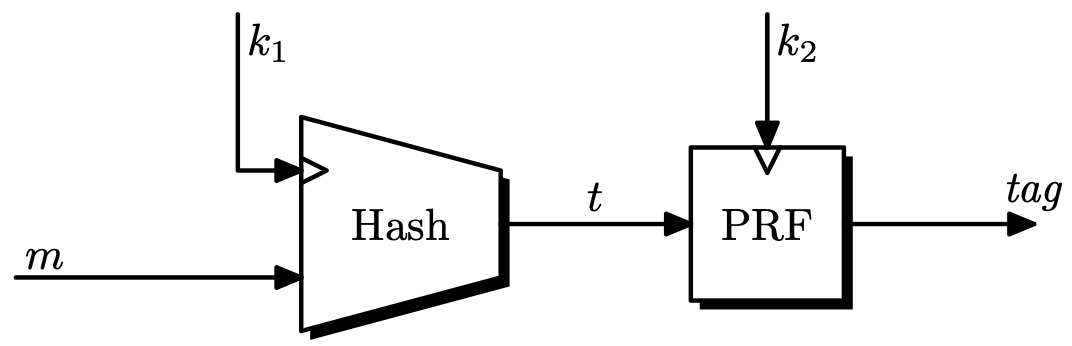
\includegraphics[width=0.45\linewidth]{figures/chapter7/fig1.png}
  \caption{先哈希后 PRF 范式}
  \label{fig:7-1}
\end{figure}

\section{通用哈希函数}
\section{构造 UHF}\label{sec:7-2}

构建良好的通用哈希函数(UHF)的挑战是构建一个使用短密钥实现小碰撞概率的函数。最理想的情况是密钥的长度不取决与被哈希的消息的长度。我们下面给出三种构造。第一种构造是基于算术模运算和多项式的一个\emph{统计性} UHF 的优雅构造。第二种构造基于 \ref{sec:6-4} 节中介绍的 CBC 和级联函数。我们表明,这两者都是\emph{计算性} UHF。第三种构造基于 \ref{sec:6-11} 节中介绍的 $\mathrm{PMAC}_0$。

\subsection{构造 1:使用多项式构建 UHF}\label{subsec:7-2-1}

我们从一个使用多项式模一个素数的 UHF 构造开始。令 $\ell$ 是一个(多项式边界的)长度参数,并令 $p$ 是一个素数。我们定义一个哈希函数 $H_{\rm poly}$,它能将一条消息 $m\in\mathbb{Z}^{\leq\ell}_p$ 哈希为一个单一元素 $t\in\mathbb{Z}_p$。其密钥空间为 $\mathcal{K}:=\mathbb{Z}_p$。

令 $m$ 是一条消息,即 $m=(a_1,\dots,a_v)\in\mathbb{Z}^{\leq\ell}_p$,其中 $0\leq v\leq\ell$。令 $k\in\mathbb{Z}_p$ 是一个密钥。哈希函数 $H_{\rm poly}(k,m)$ 的定义如下:
\begin{equation}\label{eq:7-3}
H_{\rm poly}\big(k,\,(a_1,\dots,a_v)\big)=k^v+a_1k^{v-1}+a_2k^{v-2}+\cdots+a_{v-1}k+a_v\in\mathbb{Z}_p
\end{equation}
也就是说,我们使用 $(1,a_1,a_2,\dots,a_v)$ 作为一个 $v$ 阶多项式 $f(X)$ 的系数向量,然后在一个秘密点 $k$ 处评估 $f(X)$。

这个哈希函数的一个非常有用的特性是,它可以在不提前知道消息长度的情况下进行评估。我们可以随时在消息分组可用时将其输入到哈希函数中。当消息结束时,我们会得到最终的哈希值。我们使用 Horner 的多项式评估方法来实现这一点:

\vspace{5pt}

\hspace*{5pt} 输入:消息 $m=(a_1,\dots,a_v)\in\mathbb{Z}^{\leq\ell}_p$ 和密钥 $k\in\mathbb{Z}_p$\\
\hspace*{26pt} 输出:$t=H_{\rm poly}(k,m)$

\vspace{5pt}

\hspace*{5pt} 1. \quad 置 $t\leftarrow1$\\
\hspace*{26pt} 2. \quad 对于 $i=1,\dots,v$:\\
\hspace*{26pt} 3. \quad\quad\quad 令 $t\leftarrow t\cdot k+a_i\in\mathbb{Z}_p$\\
\hspace*{26pt} 4. \quad 输出 $t$

\vspace{5pt}

\noindent
不难看出,这种算法产生的数值与式 \ref{eq:7-3} 中定义的相同。观察到,对于一条长消息,我们可以使用很少的额外空间来一次处理一个分组。每次迭代都只需要一次乘法和一次加法。
 
在包含多个乘法单元——比如四个——的机器上,我们可以使用 Horner 方法的 $4$ 路并行版本来加快 $H_{\rm poly}$ 的评估速度。假设 $m$ 的长度是 $4$ 的倍数,我们只需将上面的第 $2$ 行和第 $3$ 行替换为以下内容:

\vspace{5pt}

\hspace*{5pt} 2. \quad 对于 $i=1,\dots,v$,每次迭代将 $i$ 递增 $4$:\\
\hspace*{26pt} 3. \quad\quad\quad 令 $t\leftarrow t\cdot k^4+a_i\cdot k^3+a_{i+1}\cdot k^2+a_{i+2}\cdot k+a_{i+3}\;\in\mathbb{Z}_p$

\vspace{5pt}

\noindent
我们可以预先计算 $\mathbb{Z}_p$ 上的 $k_2$,$k_3$ 和 $k_4$。然后,在每次迭代中,我们都并行地执行四个乘法计算来处理四个消息分组。

\begin{snote}[作为一个 UHF 的安全性。]
接下来我们表明,$H_{\rm poly}$ 是一个 ${(\ell/p)}$-UHF。如果 $p$ 是超多项式的,这就意味着 ${(\ell/p)}$ 可忽略不计,也就意味着 $H_{\rm poly}$ 是一个统计性 UHF。
\end{snote}

\begin{lemma}\label{lemma:7-2}
式 \ref{eq:7-3} 中定义的 $(\mathbb{Z}_p,(\mathbb{Z}_p)^{\leq\ell},\mathbb{Z}_p)$ 上的函数 $H_{\rm poly}$ 是一个 ${(\ell/p)}$-UHF。
\end{lemma}

\begin{proof}
考虑 $(\mathbb{Z}_p)^{\leq\ell}$ 中的两条互不相同的消息 $m_0=(a_1,\dots,a_u)$  和 $m_1=(b_1,\dots,b_v)$。我们想要说明 $\Pr[H_{\rm poly} (k,m_0) = H_{\rm poly} (k,m_1)] \leq {\ell/q}$,其中的概率基于从 $\mathbb{Z}_p$ 中随机选择的密钥 $k$。定义 $\mathbb{Z}_p[X]$ 上的两个多项式:
\begin{equation}	\label{eq:7-4}
\begin{aligned}
& f(X):=X^u+a_1X^{u-1}+a_2X^{u-2}+\cdots+a_{u-1}X+a_u\\
& g(X):=X^v+b_1X^{v-1}+b_2X^{v-2}+\cdots+b_{v-1}X+b_v
\end{aligned}
\end{equation}
于是,根据 $H_{\rm poly}$ 的定义,我们需要证明:
\[
\Pr[f(k)=g(k)]\leq{\ell/p}
\]
其中,$k$ 均匀分布在 $\mathbb{Z}_p$ 上。换句话说,我们需要限定使得 $f(k)-g(k)=0$ 成立的点 $k\in\mathbb{Z}_p$ 的数量。由于 $m_0$ 和 $m_1$ 互不相同,所以 $f(X)-g(X)$ 是一个非零的多项式。此外,该多项式最高为 $\ell$ 阶,因此它在 $\mathbb{Z}_p$ 上最多有 $\ell$ 个根。于是,最多有 $\ell$ 个 $k\in\mathbb{Z}_p$ 使得 $f(k)=g(k)$ 成立,因而,对于一个随机的 $k\in\mathbb{Z}_p$,必然有 $\Pr[f(k)=g(k)]\leq{\ell/p}$ 成立,满足要求。
\end{proof}

\begin{snote}[为什么 $H_{\rm poly}(k,m)$ 的首项是 $k^v$?]
在式 \ref{eq:7-3} 中,对 $H_{\rm poly}(k,m)$ 的定义包括一个首项 $k^v$,该项确保该函数是一个适用于变长输入的统计性 UHF。如果我们在定义 $H_{\rm fpoly}(k,m)$ 时不包含该项,即: 
\begin{equation}\label{eq:7-5}
H_{\rm fpoly}\big(k,\,(a_1,\dots,a_v)\big):=a_1k^{v-1}+a_2k^{v-2}+\cdots+a_{v-1}k+a_v\in\mathbb{Z}_p
\end{equation}
那么对于变长输入来说,其结果就不是 UHF。比如说,以下两条消息 $m_0=(a_1,a_2)\in\mathbb{Z}^2_p$ 和 $m_1=(0,a_1,a_2)\in\mathbb{Z}^3_p$ 在所有的密钥 $k\in\mathbb{Z}_p$ 下都是对 $H_{\rm fpoly}$ 的碰撞。尽管如此,在练习 \ref{exer:7-16} 中,我们将会表明,如果我们把 $H_{\rm fpoly}$ 的输入空间限制在定长的消息上,比如 $\mathcal{M}:=\mathbb{Z}_p^\ell$,那么它仍然是一个统计性 UHF。更具体地说,$H_{\rm fpoly}$ 是一个 $(\ell-1)/p$-UHF。相比之下,式 \ref{eq:7-3} 中定义的函数 $H_{\rm fpoly}$ 对于包含变长输入的输入空间 $\mathbb{Z}_p^\ell$ 来说是一个统计性 UHF。
\end{snote}

\begin{remark}\label{remark:7-1}
函数 $H_{\rm poly}$ 接受 $\mathbb{Z}^{\leq\ell}_p$ 中的输入,并输出 $\mathbb{Z}_p$ 上的值。这并不是十分理想,因为我们更倾向于使用对长为 $n$ 比特的分组进行操作的函数,其中的 $n$ 是某个正整数。我们可以调整式 \ref{eq:7-3} 中对 $H_{\rm poly}$ 的定义,使其不在 $\mathbb{Z}_p$ 上工作,而是在有限域 ${\rm GF}(2^n)$ 上进行算术运算。使用与引理 \ref{lemma:7-2} 完全相同的分析方法,我们可以看到,这个版本的 $H_{\rm poly}$ 是一个 ${(/2^n)}$-UHF。它输出 ${\rm GF}(2^n)$ 上的值。在练习 \ref{exer:7-1} 中,我们将会表明,简单地将 $H_{\rm poly}$ 定义为模 $2^n$ 运算(即工作在 $\mathbb{Z}_{2^n}$ 上)将得到一个完全不安全的 UHF。
\end{remark}

\begin{snote}[使用 UHF 时的注意事项。]
UHF 可能很脆弱——一个对手如果知道了函数在几个点上的值,就完全有可能回复密钥。例如,$H_{\rm poly}(k,\cdot)$ 在一个点上的值就会完全暴露密钥 $k\in\mathbb{Z}_p$。事实上,如果 $m=(a_1)$,由于 $H_{\rm poly}(k,m)=k+a_1$,那么同时拥有 $m$ 和 $H_{\rm poly}(k,m)$ 的对手立即就能得到 $k\in\mathbb{Z}_p$。因此,在我们对 UHF 的所有应用中,我们都必须始终通过加密或者其他方式向对手隐藏 UHF 的值。
\end{snote}

\begin{snote}[数学细节。]
$H_{\rm poly}$ 的定义需要一个素数 $p$。到目前为止,我们只是假设 $p$ 是一个在最开始时选取的公共值,并且永远固定。在正式的 UHF 框架(见 \ref{subsec:7-1-2} 小节)中,素数 $p$ 是一个系统参数,用 $\Lambda$ 来表示。它由一个\emph{系统参数生成算法} $P$ 生成,该算法将安全参数 $\lambda$ 作为输入,并输出某个素数 $p$。

更确切地说,令 $L:\mathbb{Z}\to\mathbb{Z}$ 是某个将安全参数映射到指定比特长度的素数的函数。那么 $H_{\rm poly}$ 的正式定义应当包括对算法 $P$ 的描述,它将安全参数 $\lambda$ 作为输入,并输出一个长度为 $L(\lambda)$ 的素数 $p$。具体地,$\Lambda:=p$,并且:
\[
\mathcal{K}_{\lambda,p}=\mathbb{Z}_p,
\quad\quad
\mathcal{M}_{\lambda,p}=\mathbb{Z}^{\leq\ell(\lambda)},
\quad\quad
\mathcal{T}_{\lambda,p}=\mathbb{Z}_p
\]
其中 $\ell:\mathbb{Z}\to\mathbb{Z}^{\geq0}$ 是多项式边界的。根据引理 \ref{lemma:7-2},我们可知:
\[
{\rm UHF}\mathsf{adv}[\mathcal{A},H_{\rm poly}](\lambda)\leq{\ell(\lambda)}/{2^{L(\lambda)}}
\]
只要 $2^{L(\lambda)}$ 是超多项式的,上式就是一个 $\lambda$ 的可忽略不计函数。
\end{snote}

\subsection{构造2:CBC 和级联都是计算性 UHF}\label{subsec:7-2-2}

接下来,我们表明,\ref{sec:6-4} 节中所定义的 CBC 和级联构造都是计算性 UHF。更一般地,我们表明,任何可扩展的无前缀安全 PRF 都是计算性 UHF。回顾一下,如果对于所有的 $k\in\mathcal{K}$,$x,y\in\mathcal{X}^{\leq\ell-1}$ 和 $a\in\mathcal{X}$,我们都有:
\[
\text{如果}\quad
F(k,x)=F(k,y)
\quad\text{则}\quad
F(k,\;x\,\Vert\,a)=F(k,\;y\,\Vert\,a)
\]
那么定义在 $(\mathcal{K},\mathcal{X}^{\leq\ell},\mathcal{Y})$ 上的 PRF $F$ 就是可扩展的。在上一章中,我们已经证明了 CBC 和级联构造都是无前缀安全 PRF,并且两者都是可扩展的。

\begin{theorem}\label{theo:7-3}
令 $PF$ 是一个定义在 $(\mathcal{K},\mathcal{X}^{\leq\ell+1},\mathcal{Y})$ 上的可扩展的,且无前缀安全的 PRF,其中 $|\mathcal{Y}|$ 是超多项式的,且 $|\mathcal{X}|>1$。那么 $PF$ 也是一个定义在 $(\mathcal{K},\mathcal{X}^{\leq\ell},\mathcal{Y})$ 上的计算性 UHF。
\begin{quote}
特别地,对于每个就 $PF$ 进行攻击游戏 \ref{game:7-1} 的 UHF 对手 $\mathcal{A}$,都必然存在一个无前缀 PRF 对手 $\mathcal{B}$,其中 $\mathcal{B}$ 是一个围绕 $\mathcal{A}$ 的基本包装器,满足:
\end{quote}
\begin{equation}\label{eq:7-6}
{\rm UHF}\mathsf{adv}[\mathcal{A},PF]\leq{\rm PRF^{pf}}\mathsf{adv}[\mathcal{B},PF]+\frac{1}{|\mathcal{Y}|}
\end{equation}
\begin{quote}
此外,$\mathcal{B}$ 只会对 $PF$ 发起两次查询。
\end{quote}
\end{theorem}

\begin{proof}
令 $\mathcal{A}$ 是一个攻击 $PF$ 的 UHF 对手。我们下面构造一个攻击 $PF$ 的无前缀 PRF 对手 $\mathcal{B}$。$\mathcal{B}$ 在攻击游戏 \ref{game:4-2} 中扮演对手,它的目标是区分实验 $0$ 和实验 $1$,在实验 $0$ 中,它用一个随机数 $k\in\mathcal{K}$ 查询一个函数 $f\leftarrow PF(k,\cdot)$,而在实验 $1$ 中,它查询一个随机函数 $f\overset{\rm R}\leftarrow{\rm Funs}[\mathcal{X}^{\leq\ell+1},\mathcal{Y}]$。

首先,我们给出一些关于 $\mathcal{B}$ 如何工作的直觉。$\mathcal{B}$ 从运行 UHF 对手 $\mathcal{A}$ 开始,获得两条不同消息 $m_0,m_1\in\mathcal{X}^{\leq\ell}$。根据 $\mathcal{A}$ 的定义,我们知道,在实验 $0$ 中,我们有:
\[
\Pr[f(m_0)=f(m_1)]={\rm UHF}\mathsf{adv}[\mathcal{A},PF]
\]
而在实验 $1$ 中,由于 $f$ 是一个随机函数,并且 $m_0\neq m_1$,我们有:
\[
\Pr[f(m_0)=f(m_1)]={1}/{|\mathcal{Y}|}
\]
因此,如果 $\mathcal{B}$ 能在 $m_0$ 和 $m_1$ 处查询 $f$,它就能以 $\big\lvert{\rm UHF}\mathsf{adv}[\mathcal{A},PF]-{1}/{|\mathcal{Y}|}\big\rvert$ 的优势区分这两个实验,这就证明了该定理。

不幸的是,对 $\mathcal{B}$ 的这种设计并不奏效,因为 $m_0$ 可能是 $m_1$ 的一个真前缀。在这种情况下,$\mathcal{B}$ 不会被允许在 $m_0$ 和 $m_1$ 处查询 $f$,因为 $\mathcal{B}$ 应当是一个无前缀对手。然而,可扩展的属性提供了一个简单的解决方案:我们可以在 $m_0$ 和 $m_1$ 之后各附加一个分组 $a\in\mathcal{X}$,这样 $m_0\,\Vert\,a$ 就不再是 $m_1\,\Vert\,a$ 的真前缀了。如果 $m_0=(a_1,\dots,a_u)$,$m_1=(b_1,\dots,b_v)$,那么任何的 $a\neq b_{u+1}$ 都能解决这个问题。此外,根据可扩展属性,我们知道:
\[
PF(k,\,m_0)=PF(k,\,m_1)
\quad\Longrightarrow\quad
PF(k,\,m_0\,\Vert\,a)=PF(k,\,m_1\,\Vert\,a)
\]
由于 $m_0\,\Vert\,a$ 不再是 $m_1\,\Vert\,a$ 的真前缀,所以我们的 $\mathcal{B}$ 可以对这两个输入查询 $f$。于是,$\mathcal{B}$ 在区分实验 $0$ 和实验 $1$ 方面就能够获得预期的优势。

更详细地说,$\mathcal{B}$ 的工作流程如下:

\vspace{5pt}

\hspace*{5pt} 运行 $\mathcal{A}$,获得 $\mathcal{X}^{\leq\ell}$ 上的两条互不相同的消息 $m_0$ 和 $m_1$,其中\\
\hspace*{50pt} $m_0=(a_1,\dots,a_u)$,且 $m_1=(b_1,\dots,b_v)$\\
\hspace*{26pt} 假设 $u\leq v$(否则就交换两条消息)\\
\hspace*{26pt} 如果 $m_0$ 是 $m_1$ 的真前缀:\\
\hspace*{50pt} 选择某个 $a\in\mathcal{X}$ 使得 $a\neq b_{u+1}$\\
\hspace*{50pt} 令 $m_0'\leftarrow m_0\,\Vert\,a$,$m_1'\leftarrow m_1\,\Vert\,a$\\
\hspace*{26pt} 否则:\\
\hspace*{50pt} 令 $m_0'\leftarrow m_0$,$m_1'\leftarrow m_1$\\
\hspace*{26pt} // \emph{此时,我们能够确定 $m_0'$不是$m_1'$的真前缀,反之亦然}\\
\hspace*{26pt} 在 $m_0'$ 和 $m_1'$ 处查询 $f$,得到 $t_0:=f(m_0')$ 和 $t_1:=f(m_1')$\\
\hspace*{26pt} 如果 $t_0=t_1$ 则输出 $1$,否则就输出 $0$

\vspace{5pt}

观察到 $\mathcal{B}$ 是一个无前缀 PRF 对手,且只对 $f$ 进行了两次查询,与要求一致。现在,对于 $b=0,1$,令 $p_b$ 是 $\mathcal{B}$ 在实验 $b$ 中输出 $1$ 的概率。那么,在实验 $0$ 中,我们知道:
\begin{equation}\label{eq:7-7}
p_0:=\Pr[f(m_0')=f(m_1')]\geq\Pr[f(m_0)=f(m_1)]={\rm UHF}\mathsf{adv}[\mathcal{A},PF]
\end{equation}
而在实验 $1$ 中,我们知道:
\begin{equation}\label{eq:7-8}
p_1:=\Pr[f(m_0')=f(m_1')]={1}/{|\mathcal{Y}|}
\end{equation}
因此,根据式 \ref{eq:7-7} 和 \ref{eq:7-8},我们有:
\[
{\rm PRF^{pf}}\mathsf{adv}[\mathcal{B},PF]=|p_0-p_1|\geq p_0-p_1\geq{\rm UHF}\mathsf{adv}[\mathcal{A},PF]-{1}/{|\mathcal{Y}|}
\]
由此可得式 \ref{eq:7-6} 成立。
\end{proof}

\begin{snote}[$PF$ 是一个多次查询 UHF。]
引理 \ref{lemma:7-1} 表明,$PF$ 也是一个多次查询 UHF。然而,对该事实的一个直接的证明能够给出一个更好对安全上界。
\end{snote}

\begin{theorem}\label{theo:7-4}
令 $PF$ 是一个定义在 $(\mathcal{K},\mathcal{X}^{\leq\ell+1},\mathcal{Y})$ 上的可扩展的,且无前缀安全 PRF,其中 $|\mathcal{X}|$ 和 $|\mathcal{Y}|$ 都是超多项式的,且 $\ell$ 是多项式边界的。那么 $PF$ 是一个定义在 $(\mathcal{K},\mathcal{X}^{\leq\ell},\mathcal{Y})$ 上的多次查询 UHF。
\begin{quote}
特别地,如果 $|\mathcal{X}|>\ell Q$,那么对于每个 $Q$ 次查询 UHF 对手 $\mathcal{A}$,都必然存在一个 $Q$ 次查询无前缀 PRF 对手 $\mathcal{B}$,其中 $\mathcal{B}$ 是一个围绕 $\mathcal{A}$ 的基本包装器,满足:
\end{quote}
\begin{equation}\label{eq:7-9}
{\rm MUHF}\mathsf{adv}[\mathcal{A},PF]\leq{\rm PRF^{pf}} \mathsf{adv}[\mathcal{B},PF]+\frac{Q^2}{2|\mathcal{Y}|}
\end{equation}
\end{theorem}

\begin{proof}
该证明的证明与定理 \ref{theo:7-3} 的证明相似。对手 $\mathcal{B}$ 首先运行 $Q$ 次查询 UHF 对手 $\mathcal{A}$,以获得 $\mathcal{X}^{\leq\ell}$ 上的几条各不相同的消息 $m_1,\dots,m_s$,其中 $s\leq Q$。接下来,$\mathcal{B}$ 找到一个 $a\in\mathcal{X}$,使得 $a$ 不等于 $m_1,\dots,m_s$ 中的任何一个消息分组。由于 $|\mathcal{X}|$ 是超多项式的,我们可以假设它大于 $\ell Q$,因此这个 $a$ 一定存在。令 $m_i':=m_i\,\Vert\,a$,其中 $i=1,\dots,s$。于是,根据 $a$ 的定义,集合 $\{m_1',\dots,m_s'\}$ 是一个无前缀集合。无前缀对手 $\mathcal{B}$ 现在在 $m_1',\dots,m_s'$ 处向挑战者发起查询,并得到应答 $t_1,\dots,t_s$。如果存在 $i\neq j$ 使得 $t_i=t_j$,$\mathcal{B}$ 就输出 $1$,否则就输出 $0$。

为了分析 $\mathcal{B}$ 的优势,对于 $b=0,1$,我们令 $p_b$ 为 $\mathcal{B}$ 在实验 $b$ 中输出 $1$ 的概率。与式 \ref{eq:7-7} 中一样,可扩展属性意味着:
\[
p_0\geq{\rm MUHF}\mathsf{adv}[\mathcal{A},PF]
\]
在实验 $1$ 中,联合约束意味着:
\[
p_1\leq\frac{Q(Q-1)}{2|\mathcal{Y}|}
\]
因此:
\[
{\rm PRF^{pf}}\mathsf{adv}[\mathcal{B},PF]=|p_0-p_1|\geq p_0-p_1\geq{\rm MUHF}\mathsf{adv}[\mathcal{A},PF]-\frac{Q^2}{2|\mathcal{Y}|}
\]
于是,式 \ref{eq:7-9} 成立。
\end{proof}

\begin{snote}[定理 7.3 和定理 7.4 的应用。]
将定理 \ref{theo:7-4} 应用于 CBC 和级联,可以证明两者都是计算性 UHF。我们在下面的推论中将说明由此产生的误差界限,该界限可由 CBC 定理(定理 \ref{theo:6-3})和级联定理(定理 \ref{theo:6-4})中的界限推出。\footnote{请注意,定理 \ref{theo:7-4} 迫使我们在应用定理 \ref{theo:6-3} 和 \ref{theo:6-4} 时用 $\ell+1$ 来代替 $\ell$。}
\end{snote}

\begin{corollary}\label{cor:7-5}
令 $F$ 是一个定义在 $(\mathcal{K},\mathcal{X},\mathcal{Y})$ 上的安全的 PRF。那么,接受 $\mathcal{X}^{\leq\ell}$ 上的输入的 CBC 构造 $F_{\rm CBC}$(假设 $\mathcal{Y}=\mathcal{X}$ 的大小是超多项式的)和级联构造 $F^*$(假设 $\mathcal{Y}=\mathcal{K}$)对于多项式约束的 $\ell$ 都是计算性 UHF。
\begin{quote}
特别地,对于每个 $Q$ 次查询 UHF 对手 $\mathcal{A}$,必然存在两个无前缀 PRF 对手 $\mathcal{B}_1$ 和 $\mathcal{B}_2$,它们都是 $\mathcal{A}$ 的基本包装器,满足:
\end{quote}
\begin{equation}\label{eq:7-10}
{\rm MUHF}\mathsf{adv}[\mathcal{A},F_{\rm CBC}]\leq{\rm PRF^{pf}}\mathsf{adv}[\mathcal{B}_1,F]+\frac{Q^2(\ell+1)^2+Q^2}{2|\mathcal{Y}|}
\end{equation}
\begin{quote}
和
\end{quote}
\begin{equation}\label{eq:7-11}
{\rm MUHF}\mathsf{adv}[\mathcal{A},F^*]\leq Q(\ell+1)\cdot{\rm PRF^{pf}}\mathsf{adv}[\mathcal{B}_2,F]+\frac{Q^2}{2|\mathcal{Y}|}
\end{equation}
\end{corollary}

\noindent
在式 \ref{eq:7-10} 和 \ref{eq:7-11} 中令 $Q:=2$,可以得到作为 UHF 的 $F_{\rm CBC}$ 和 $F^*$ 的误差上界。

\subsection{构造 3:使用小的 PRF 构建的一种并行 UHF}\label{subsec:7-2-3}

CBC 和级联构造都能从小领域的 PRF 中产生高效的 UHF,但是它们本身都是串行性的,因而无法利用硬件的并行性。幸运的是,从一个小领域的 PRF 中构造一个适用于并行架构的 UHF 并不困难。一个被称为异或哈希(XOR-hash)的例子,用$F^\oplus$ 表示,如图 \ref{fig:7-2} 所示。异或哈希定义在 $(\mathcal{K},\mathcal{X}^{\leq\ell},\mathcal{Y})$ 上,其中 $\mathcal{Y}=\{0,1\}^n$,并且是由一个定义在 $(\mathcal{K},\mathcal{X}\times\{1,\dots,\ell\},\mathcal{Y})$ 上的 PRF $F$ 构建来的。异或哈希的工作方式如下:

\begin{figure}
  \centering
  

\tikzset{every picture/.style={line width=0.75pt}} %set default line width to 0.75pt        

\begin{tikzpicture}[x=0.75pt,y=0.75pt,yscale=-1,xscale=1]
%uncomment if require: \path (0,212); %set diagram left start at 0, and has height of 212

%Shape: Rectangle [id:dp3703164431038082] 
\draw  [fill={rgb, 255:red, 255; green, 255; blue, 255 }  ,fill opacity=1 ][line width=1.2] [general shadow={fill=black,shadow xshift=2.25pt,shadow yshift=-2.25pt}] (0,0.5) -- (70,0.5) -- (70,20.5) -- (0,20.5) -- cycle ;
%Straight Lines [id:da2288818424042205] 
\draw    (35,20) -- (35,45.5) ;
\draw [shift={(35,48.5)}, rotate = 270] [fill={rgb, 255:red, 0; green, 0; blue, 0 }  ][line width=0.08]  [draw opacity=0] (7.14,-3.43) -- (0,0) -- (7.14,3.43) -- cycle    ;
%Shape: Rectangle [id:dp38434692876948917] 
\draw  [fill={rgb, 255:red, 255; green, 255; blue, 255 }  ,fill opacity=1 ][line width=1.2] [general shadow={fill=black,shadow xshift=2.25pt,shadow yshift=-2.25pt}] (90,0) -- (160,0) -- (160,20) -- (90,20) -- cycle ;
%Straight Lines [id:da5188910523623944] 
\draw    (125,20) -- (125,45.5) ;
\draw [shift={(125,48.5)}, rotate = 270] [fill={rgb, 255:red, 0; green, 0; blue, 0 }  ][line width=0.08]  [draw opacity=0] (7.14,-3.43) -- (0,0) -- (7.14,3.43) -- cycle    ;
%Shape: Rectangle [id:dp3329124039509572] 
\draw  [fill={rgb, 255:red, 255; green, 255; blue, 255 }  ,fill opacity=1 ][line width=1.2] [general shadow={fill=black,shadow xshift=2.25pt,shadow yshift=-2.25pt}] (180,0) -- (250,0) -- (250,20) -- (180,20) -- cycle ;
%Straight Lines [id:da9982393046561384] 
\draw    (215,20.5) -- (215,46) ;
\draw [shift={(215,49)}, rotate = 270] [fill={rgb, 255:red, 0; green, 0; blue, 0 }  ][line width=0.08]  [draw opacity=0] (7.14,-3.43) -- (0,0) -- (7.14,3.43) -- cycle    ;
%Shape: Rectangle [id:dp5817171685461355] 
\draw  [fill={rgb, 255:red, 255; green, 255; blue, 255 }  ,fill opacity=1 ][line width=1.2] [general shadow={fill=black,shadow xshift=2.25pt,shadow yshift=-2.25pt}] (310,0) -- (380,0) -- (380,20) -- (310,20) -- cycle ;
%Straight Lines [id:da43116016737929086] 
\draw    (345,20) -- (345,45.5) ;
\draw [shift={(345,48.5)}, rotate = 270] [fill={rgb, 255:red, 0; green, 0; blue, 0 }  ][line width=0.08]  [draw opacity=0] (7.14,-3.43) -- (0,0) -- (7.14,3.43) -- cycle    ;
%Straight Lines [id:da13149857378263796] 
\draw    (35,90) -- (35,105) -- (180.08,139.31) ;
\draw [shift={(183,140)}, rotate = 193.31] [fill={rgb, 255:red, 0; green, 0; blue, 0 }  ][line width=0.08]  [draw opacity=0] (7.14,-3.43) -- (0,0) -- (7.14,3.43) -- cycle    ;
%Straight Lines [id:da8567076780252318] 
\draw    (125,90) -- (125,105) -- (185.29,133.71) ;
\draw [shift={(188,135)}, rotate = 205.46] [fill={rgb, 255:red, 0; green, 0; blue, 0 }  ][line width=0.08]  [draw opacity=0] (7.14,-3.43) -- (0,0) -- (7.14,3.43) -- cycle    ;
%Straight Lines [id:da4177163318233448] 
\draw    (215,90) -- (215,105) -- (193.83,132.62) ;
\draw [shift={(192,135)}, rotate = 307.48] [fill={rgb, 255:red, 0; green, 0; blue, 0 }  ][line width=0.08]  [draw opacity=0] (7.14,-3.43) -- (0,0) -- (7.14,3.43) -- cycle    ;
%Straight Lines [id:da08439238562392437] 
\draw    (345,90) -- (345,105) -- (199.92,139.31) ;
\draw [shift={(197,140)}, rotate = 346.69] [fill={rgb, 255:red, 0; green, 0; blue, 0 }  ][line width=0.08]  [draw opacity=0] (7.14,-3.43) -- (0,0) -- (7.14,3.43) -- cycle    ;
%Straight Lines [id:da12566654354732099] 
\draw    (190,145) -- (190,177) ;
\draw [shift={(190,180)}, rotate = 270] [fill={rgb, 255:red, 0; green, 0; blue, 0 }  ][line width=0.08]  [draw opacity=0] (7.14,-3.43) -- (0,0) -- (7.14,3.43) -- cycle    ;
%Shape: Trapezoid [id:dp0005402873648003848] 
\draw  [fill={rgb, 255:red, 255; green, 255; blue, 255 }  ,fill opacity=1 ][line width=1.2] [general shadow={fill=black,shadow xshift=2.25pt,shadow yshift=-2.25pt}] (70,50) -- (58,90) -- (12,90) -- (0,50) -- cycle ;
%Shape: Trapezoid [id:dp2231918842135976] 
\draw  [fill={rgb, 255:red, 255; green, 255; blue, 255 }  ,fill opacity=1 ][line width=1.2] [general shadow={fill=black,shadow xshift=2.25pt,shadow yshift=-2.25pt}] (160,50) -- (148,90) -- (102,90) -- (90,50) -- cycle ;
%Shape: Trapezoid [id:dp8197321821978614] 
\draw  [fill={rgb, 255:red, 255; green, 255; blue, 255 }  ,fill opacity=1 ][line width=1.2] [general shadow={fill=black,shadow xshift=2.25pt,shadow yshift=-2.25pt}] (250,50) -- (238,90) -- (192,90) -- (180,50) -- cycle ;
%Shape: Trapezoid [id:dp6599035304294065] 
\draw  [fill={rgb, 255:red, 255; green, 255; blue, 255 }  ,fill opacity=1 ][line width=1.2] [general shadow={fill=black,shadow xshift=2.25pt,shadow yshift=-2.25pt}] (380,50) -- (368,90) -- (322,90) -- (310,50) -- cycle ;

% Text Node
\draw (35,70) node  [font=\small]  {$F( k ,\cdot )$};
% Text Node
\draw (35,10.5) node  [font=\small]  {$( a_{1} ,\ 1)$};
% Text Node
\draw (125,10) node  [font=\small]  {$( a_{2} ,\ 2)$};
% Text Node
\draw (215,10) node  [font=\small]  {$( a_{3} ,\ 3)$};
% Text Node
\draw (345,10) node  [font=\small]  {$( a_{v} ,\ v)$};
% Text Node
\draw (190,140) node  [font=\large]  {$\oplus $};
% Text Node
\draw (125,70) node  [font=\small]  {$F( k ,\cdot )$};
% Text Node
\draw (215,70) node  [font=\small]  {$F( k ,\cdot )$};
% Text Node
\draw (345,70) node  [font=\small]  {$F( k ,\cdot )$};
% Text Node
\draw (192,180) node [anchor=west] [inner sep=0.75pt]  [font=\small]  {$F^{\oplus }( k ,m)$};
% Text Node
\draw (280,10) node    {$\cdots $};
% Text Node
\draw (280,70) node    {$\cdots $};


\end{tikzpicture}
  \caption{一个来自小 PRF 的并行 PRF}
  \label{fig:7-2}
\end{figure}

\vspace{5pt}

\hspace*{5pt} 输入:$k\in\mathcal{K}$ 和 $m=(a_1,\dots,a_v)\in\mathcal{X}^{\leq\ell}$,其中 $0\leq v\leq\ell$\\
\hspace*{26pt} 输出:一个 $\mathcal{Y}$ 中的标签

\vspace{5pt}

\hspace*{5pt} 令 $t\leftarrow0^n$\\
\hspace*{26pt} 对于 $i=1,\dots,v$:\\
\hspace*{50pt} 令 $t\leftarrow t\oplus F(k,\,(a_i,i))$\\
\hspace*{26pt} 输出 $t$

\vspace{5pt}

\noindent
对 $F^\oplus$ 的评估可以很容易地以并行的方式完成。下面的定理表明,$F^\oplus$ 是一个计算性 UHF。请注意,与我们之前介绍的 UHF 构造不同,$F^\oplus$ 的安全性不取决于输入消息的长度。在下一节中,我们将使用 $F^\oplus$ 来构建一个适用于并行架构的安全的 MAC。

\begin{theorem}\label{theo:7-6}
令 $F$ 是一个安全的 PRF,并且 $|\mathcal{Y}|$ 是超多项式的。那么 $F^\oplus$ 是一个计算性 UHF。
\begin{quote}
特别地,对于每个 UHF 对手 $\mathcal{A}$,都必然存在一个 PRF 对手 $\mathcal{B}$,其中 $\mathcal{B}$ 是一个围绕 $\mathcal{A}$ 的基本包装器,满足:
\end{quote}
\begin{equation}\label{eq:7-12}
{\rm UHF}\mathsf{adv}[\mathcal{A},F^\oplus]\leq{\rm PRF}\mathsf{adv}[\mathcal{B},F]+\frac{1}{|\mathcal{Y}|}
\end{equation}
\end{theorem}

\begin{proof}
该证明是一个由两个游戏组成的序列。

\vspace{5pt}

\noindent\textbf{游戏 $\mathbf{0}$}。
该游戏的挑战者计算:

\vspace{5pt}

\hspace*{5pt} 选取 $k\overset{\rm R}\leftarrow\mathcal{K}$,令 $f\leftarrow F(k,\cdot)$

\vspace{5pt}

\noindent
对手输出 $\mathcal{X}^{\leq\ell}$ 中的两条互不相同的消息 $U$ 和 $V$。令 $u:=|U|$,$v:=|V|$。定义 $W_0$ 为在游戏 $0$ 中,条件:
\begin{equation}\label{eq:7-13}
\bigoplus_{i=0}^{u-1}f(U[i],i)=\bigoplus_{j=0}^{v-1}f(V[j],j)
\end{equation}
成立的事件。显然,我们有:
\begin{equation}\label{eq:7-14}
\Pr[W_0]={\rm UHF}\mathsf{adv}[\mathcal{A},F^\oplus]
\end{equation}

\noindent\textbf{游戏 $\mathbf{1}$}。
我们打出``PRF牌",将挑战者的计算修改为:

\vspace{5pt}

\hspace*{5pt} 选取 $f\overset{\rm R}\leftarrow{\rm Funs}[\mathcal{X}\times\{1,\dots,\ell\},\mathcal{Y}]$

\vspace{5pt}

\noindent
我们定义 $W_1$ 为在游戏 $1$ 中,式 \ref{eq:7-13} 中的条件成立的事件。

同之前一样,存在一个 PRF 对手 $\mathcal{B}$ 使得:
\begin{equation}\label{eq:7-15}
\big\lvert\Pr[W_0]-\Pr[W_1]\big\rvert\leq{\rm PRF}\mathsf{adv}[\mathcal{B},F]
\end{equation}

\noindent
证明的关键在于约束 $\Pr[W_1]$,即约束式 \ref{eq:7-13} 对消息 $U$ 和 $V$ 成立的概率。不妨假设 $u\geq v$,并在必要时调换 $U$ 和 $V$。不难发现,由于 $U$ 和 $V$ 是互不相同的两条消息,那么一定存在一个索引 $i^*$,使得式 \ref{eq:7-13} 中左侧的数对 $(U[i^*],i^*)$ 不会出现在右侧的数对 $(V[j],j)$ 中:如果 $u>v$,那么令 $i^*=u-1$ 即可完成任务;否则,如果 $u=v$,那么一定存在某个 $i^*$,使得 $U[i^*]\neq V[i^*]$,那么该 $i^*$ 就能完成任务。

我们可以将式 \ref{eq:7-13} 改写为:
\begin{equation}\label{eq:7-16}
f(U[i^*],i^*)=\bigoplus_{i\neq i^*}f(U[i],i)\ \ \oplus\ \ \bigoplus_jf(V[j],j)
\end{equation}
由于式 \ref{eq:7-16} 的左右两侧相互独立,并且左侧均匀分布在 $\mathcal{Y}$ 上,所以等号成立的概率为 ${1}/{|\mathcal{Y}|}$。由此可得:
\begin{equation}\label{eq:7-17}
\Pr[W_1]={1}/{|\mathcal{Y}|}
\end{equation}
于是,根据式 \ref{eq:7-14},\ref{eq:7-15} 和 \ref{eq:7-17},定理得证。
\end{proof}

在练习 \ref{exer:7-27} 中,我们将对定理 \ref{theo:7-6} 进行推广,得到 $F^\oplus$ 作为一个多次查询 UHF 的约束。
\section{PRF(UHF)组合:使用 UHF 构建 MAC}
\section{Carter-Wegman MAC}\label{sec:7-4}

在本节中,我们将提出一个和之前不同的范式来构建安全的 MAC 系统。与 PRF(UHF) 组合相比,这个范式能够提供另一种权衡。

回顾一下,在 PRF(UHF) 组合中,当使用 $\epsilon$-UHF 时,对手在看到 $Q$ 个签名消息后,破解 MAC 的优势会增长到 $\epsilon\cdot{Q^2}/{2}$。因此,为了确保签名多条消息时的安全性,$\epsilon$-UHF 的 $\epsilon$ 必须足够小,以便使 $\epsilon\cdot{Q^2}/{2}$ 也很小。但这也可能会损害像 $H_{\rm poly}$ 这样的 $\epsilon$-UHF 的性能,因为 $\epsilon$ 越小,哈希函数的计算速度就越慢。比如说,假设我们要求在签署了 $Q=2^{32}$ 条消息后,对手破解 MAC 的优势仍然不超过 $2^{-64}$,那么 $\epsilon$ 的值最大就只能是 ${1}/{2^{127}}$。

我们的第二个 MAC 范式,称为 Carter-Wegman MAC,保持了与 PRF(UHF) 组合相同的安全级别,但是 $\epsilon$ 要大得多。在参数和上面的例子相同的情况下,$\epsilon$ 只需要是 ${1}/{2^{64}}$。这可以显著提升哈希函数的计算速度,尤其是在消息很长的情况下。但是,该构造的缺点是所产生的标签可能比 PRF(UHF) 组合所产生的标签要长。在练习 7.5 中,我们将探索另一种随机化的 MAC 构造,它在 $\epsilon$ 相同的条件下实现了与 Carter-Wegman MAC 相同的安全性,但是生成的标签可以更短。

Carter-Wegman MAC 是我们的第一个随机化 MAC 系统实例。它的签名算法是随机性的,也就是说,每条消息都对应着许多条合法的标签。

\vspace{5pt}

为了描述 Carter-Wegman MAC,我们首先固定某个大整数 $N$,并设置 $\mathcal{T}:=\mathbb{Z}_N$,即大小是 $N$ 的群,且群中的加法被定义为``模 $N$" 的算术运算。我们使用一个哈希函数 $H$ 和一个输出为 $\mathbb{Z}_N$ 上的元素的 PRF $F$:
\begin{itemize}
	\item $H$ 是一个定义在 $(\mathcal{K}_H,\mathcal{M},\mathcal{T})$ 上的带密钥哈希函数,
	\item $F$ 是一个定义在 $(\mathcal{K}_F,\mathcal{R},\mathcal{T})$ 上的 PRF。
\end{itemize}
Carter-Wegman MAC,表示为 $\mathcal{I}_{\rm CW}$,接受 $\mathcal{M}$ 上的元素作为输入,输出 $\mathcal{R}\times\mathcal{T}$ 中的标签。它使用 $\mathcal{K}_H\times\mathcal{K}_F$ 中的密钥。由 \textbf{$F$ 和 $H$ 派生的 Carter-Wegman MAC} 的工作原理如下(另见图 \ref{fig:7-4}):
\begin{itemize}
	\item 对于密钥 $(k_1,k_2)$ 和消息 $m$,我们定义:
	\vspace{5pt}
	
	\hspace*{5pt} $S\big((k_1,k_2),\,m\big):=$\\
	\hspace*{26pt} $r\overset{\rm R}\leftarrow\mathcal{R}$\\
	\hspace*{26pt} $v\leftarrow H(k_1,m)+F(k_2,r)\quad\in\mathbb{Z}_N$
	\quad\quad// \emph{模}$N$\emph{加法}\\
	\hspace*{26pt} 输出 $(r, v)$
	\item 对于密钥 $(k_1,k_2)$,消息 $m$ 和标签 $(r,v)$,我们定义:
	\vspace{5pt}
	
	\hspace*{5pt} $V\big((k_1,k_2),\,m,\,(r,v)\big):=$\\
	\hspace*{26pt} $v^*\leftarrow H(k_1,m)+F(k_2,r)\quad\in\mathbb{Z}_N$
	\quad\;\;// \emph{模}$N$\emph{加法}\\
	\hspace*{26pt} 如果 $v=v^*$ 就输出 $\mathsf{accept}$,否则输出 $\mathsf{reject}$
\end{itemize}

\begin{figure}
	\centering
	

\tikzset{every picture/.style={line width=0.75pt}} %set default line width to 0.75pt        

\begin{tikzpicture}[x=0.75pt,y=0.75pt,yscale=-1,xscale=1]
%uncomment if require: \path (0,130); %set diagram left start at 0, and has height of 130

%Shape: Rectangle [id:dp2935009799961412] 
\draw  [fill={rgb, 255:red, 255; green, 255; blue, 255 }  ,fill opacity=1 ][line width=1.2] [general shadow={fill=black,shadow xshift=2.25pt,shadow yshift=-2.25pt}] (270,0) -- (350,0) -- (350,80) -- (270,80) -- cycle ;
%Straight Lines [id:da9492496013009404] 
\draw    (150,40) -- (202,40) ;
\draw [shift={(205,40)}, rotate = 180] [fill={rgb, 255:red, 0; green, 0; blue, 0 }  ][line width=0.08]  [draw opacity=0] (7.14,-3.43) -- (0,0) -- (7.14,3.43) -- cycle    ;
%Shape: Trapezoid [id:dp675758013906963] 
\draw  [fill={rgb, 255:red, 255; green, 255; blue, 255 }  ,fill opacity=1 ][line width=1.2] [general shadow={fill=black,shadow xshift=2.25pt,shadow yshift=-2.25pt}] (70,0) -- (150,22.41) -- (150,57.59) -- (70,80) -- cycle ;
%Straight Lines [id:da47445358640398294] 
\draw    (0,40) -- (67,40) ;
\draw [shift={(70,40)}, rotate = 180] [fill={rgb, 255:red, 0; green, 0; blue, 0 }  ][line width=0.08]  [draw opacity=0] (7.14,-3.43) -- (0,0) -- (7.14,3.43) -- cycle    ;
%Straight Lines [id:da7362759606754594] 
\draw    (356,40) -- (420,40) ;
\draw [shift={(353,40)}, rotate = 0] [fill={rgb, 255:red, 0; green, 0; blue, 0 }  ][line width=0.08]  [draw opacity=0] (7.14,-3.43) -- (0,0) -- (7.14,3.43) -- cycle    ;
%Straight Lines [id:da8923012914951625] 
\draw    (218,40) -- (270,40) ;
\draw [shift={(215,40)}, rotate = 0] [fill={rgb, 255:red, 0; green, 0; blue, 0 }  ][line width=0.08]  [draw opacity=0] (7.14,-3.43) -- (0,0) -- (7.14,3.43) -- cycle    ;
%Straight Lines [id:da3192487827816459] 
\draw    (210,45) -- (210,97.01) ;
\draw [shift={(210,100.01)}, rotate = 270] [fill={rgb, 255:red, 0; green, 0; blue, 0 }  ][line width=0.08]  [draw opacity=0] (7.14,-3.43) -- (0,0) -- (7.14,3.43) -- cycle    ;
%Straight Lines [id:da7712844041382667] 
\draw    (380,40) -- (380,97.01) ;
\draw [shift={(380,100.01)}, rotate = 270] [fill={rgb, 255:red, 0; green, 0; blue, 0 }  ][line width=0.08]  [draw opacity=0] (7.14,-3.43) -- (0,0) -- (7.14,3.43) -- cycle    ;
%Shape: Circle [id:dp08370106862923943] 
\draw  [fill={rgb, 255:red, 0; green, 0; blue, 0 }  ,fill opacity=1 ] (378.5,40) .. controls (378.5,39.17) and (379.17,38.5) .. (380,38.5) .. controls (380.83,38.5) and (381.5,39.17) .. (381.5,40) .. controls (381.5,40.83) and (380.83,41.5) .. (380,41.5) .. controls (379.17,41.5) and (378.5,40.83) .. (378.5,40) -- cycle ;

% Text Node
\draw (2,36.6) node [anchor=south west] [inner sep=0.75pt]    {$m$};
% Text Node
\draw (110,40) node    {$H( k_{1} ,\cdot )$};
% Text Node
\draw (310,40) node    {$F( k_{2} ,\cdot )$};
% Text Node
\draw (418,36.6) node [anchor=south east] [inner sep=0.75pt]    {$r\overset{\mathrm{R}}{\leftarrow }\mathcal{R}$};
% Text Node
\draw (210,40) node  [font=\large]  {$\oplus $};
% Text Node
\draw (380,103.41) node [anchor=north] [inner sep=0.75pt]    {$r$};
% Text Node
\draw (210,103.41) node [anchor=north] [inner sep=0.75pt]    {$v$};


\end{tikzpicture}
	\caption{Carter-Wegman MAC 签名算法}
	\label{fig:7-4}
\end{figure}

Carter-Wegman 签名算法中使用了一个随机元 $r\in\mathcal{R}$。正如我们将要看到的,集合 $\mathcal{R}$ 需要足够大,以使得两条标签使用同一个随机元 $r$ 的概率可忽略不计。

\begin{snote}[一种加密 UHF MAC。]
Carter-Wegman MAC 也可以描述为对哈希函数的输出进行的一种加密。事实上,令 $\mathcal{E}=(E,D)$ 为一个密码:
\[
E(k,m):=\big\{r\overset{\rm R}\leftarrow\mathcal{R},\;\text{output }\big(r,m+F(k,r)\big)\big\}
\quad\quad\text{and}\quad\quad
D\big(k,(r,c)\big):=c-F(k,r)
\]
其中,$F$ 是一个定义在 $(\mathcal{K}_F,\mathcal{R},\mathcal{T})$ 上的 PRF。当 $F$ 是一个安全 PRF 时,这个密码是 CPA 安全的,如例 \ref{exmp:5-2} 所述。那么,Carter-Wegman MAC 可以表示为:

\vspace{5pt}

\hspace*{5pt} $S\big((k_1,k_2),\,m\big):=E\big(k_2,H(k_1,m)\big)$

\vspace{5pt}

\hspace*{5pt} $
V\big((k_1,k_2),\,m,\,t\big):=\left\{
\begin{array}{ll}
\mathsf{accept}, & \text{if }D(k_2,t)=H(k_1,m),\\
\mathsf{reject}, & \text{otherwise}
\end{array}
\right.
$

\vspace{8pt}

\noindent
我们称之为\textbf{由 $\mathcal{E}$ 和 $H$ 派生的加密 UHF MAC 系统}。

为什么要对哈希函数的输出进行加密?回顾一下,在 PRF(UHF) 组合 MAC 中,如果对手发现了两条消息 $m_1,m_2$ 在哈希函数上有碰撞(即 $H(k_1,m_1)=H(k_1,m_2)$),那么 $m_1$ 的 MAC 和 $m_2$ 的 MAC 就是一样的。因此,通过请求许多消息的标签,对手就能识别出在哈希函数上发生碰撞的消息 $m_1$ 和 $m_2$(假设在 PRF 上发生碰撞是不太可能的)。UHF 上的碰撞 $m_1,m_2$ 可以暴露出关于哈希函数密钥 $k_1$ 的信息,继而可以完全破坏 MAC。为了防止这种情况,我们必须使用一个足够小的 $\epsilon$-UHF,以确保在极高的概率下,对手永远无法找到一个哈希函数的碰撞。相对的,通过使用 CPA 安全的密码对哈希函数的输出进行加密,我们可以确保对手无法了解哈希函数在何时发生了碰撞:即使 $H(k_1,m_1)=H(k_2,m_2)$,$m_1$ 和 $m_2$ 的标签也大概率是不同的。这就使得我们可以用一个小得多的 $\epsilon$ 来维持安全性。

问题在于,即使 $(E,D)$ 是 CPA 安全的,且 $H$ 是一个 $\epsilon$-UHF,加密 UHF MAC 一般也是不安全的。例如,我们将在下面的备注 \ref{remark:7-5} 中表明,当哈希函数 $H$ 被实例化为 $H_{\rm poly}$ 时,Carter-Wegma MAC 是不安全的。为了得到一个安全的 Carter-Wegman MAC,我们需要进一步加强哈希函数 $H$,要求它满足一个更强的属性,即下面将要定义的差异不可预测性。练习 9.16 将会探讨加密 UHF MAC 的其他方面。
\end{snote}

\begin{snote}[Carter-Wegman MAC 的安全性。]
为了证明 $\mathcal{I}_\mathrm{CW}$ 的安全性,我们需要哈希函数 $H$ 满足一个比一般的 UHF 更强的属性。我们把这个更强的属性称为\textbf{差异不可预测性 (difference unpredicability)}。粗略地说,它意味着对于任意两条不同消息,预测它们哈希值的差异(在 $\mathbb{Z}_N$ 中)是很难的。和之前一样,有一个攻击游戏:
\end{snote}

\begin{game}[差异不可预测性]\label{game:7-3}
对于一个定义在 $(\mathcal{K},\mathcal{M},\mathcal{T})$ 上的带密钥哈希函数 $H$,其中 $\mathcal{T}=\mathbb{Z}_N$,以及一个给定对手 $\mathcal{A}$,攻击游戏运行如下:
\begin{itemize}
	\item 挑战者随机选取 $k\overset{\rm R}\leftarrow\mathcal{K}$,并自己保留 $k$。
	\item $\mathcal{A}$ 输出两条互不相同的消息 $m_0,m_1\in\mathcal{M}$ 和一个值 $\delta\in\mathcal{T}$。
\end{itemize}
如果 $H(k,m_1)-H(k,m_0)=\delta$,我们就称 $\mathcal{A}$ 赢得了该游戏。我们把 $\mathcal{A}$ 就 $H$ 的优势记为 ${\rm DUF}\mathsf{adv}[\mathcal{A},H]$,即 $\mathcal{A}$ 赢得该游戏的概率。
\end{game}

\begin{definition}\label{def:7-5}
令 $H$ 是一个定义在 $(\mathcal{K},\mathcal{M},\mathcal{T})$ 上的带密钥哈希函数:
\begin{itemize}
	\item 如果对于所有对手 $\mathcal{A}$(甚至是非有效的对手),都有 ${\rm DUF}\mathsf{adv}[\mathcal{A},H]\leq\epsilon$,我们就称 $H$ 是一个 \textbf{$\epsilon$-约束差异不可预测函数 ($\epsilon$-bounded difference unpredictable function)} 或 \textbf{$\epsilon$-DUF}。
	\item 如果对于某个可忽略不计的 $\epsilon$,$H$ 是一个 $\epsilon$-DUF,我们就称 $H$ 是一个\textbf{统计性 DUF}。
	\item 如果对于所有有效对手 $\mathcal{A}$,${\rm DUF}\mathsf{adv}[\mathcal{A},H]$ 都可忽略不计,我们就称 $H$ 是一个\textbf{计算性 DUF}。
\end{itemize}
\end{definition}

\begin{remark}\label{remark:7-3}
需要注意的是,由于我们定义的是一个 DUF,为了让讨论更加简单,摘要空间 $\mathcal{T}$ 必须形如 $\mathbb{Z}_N$,其中的 $N$ 是某个整数。更一般地,我们可以为一个带密钥哈希函数定义一个差异不可预测的概念,其摘要空间配备一个适当的差异算子(用抽象代数的语言来说,$\mathcal{T}$ 应该是一个\emph{阿贝尔群})。除了 $\mathbb{Z}_N$,另一个流行的摘要空间是所有 $n$ 比特序列的集合,即 $\{0,1\}^n$,相对应的差异算子为异或操作。在这种情况下,我们使用术语 \textbf{$\epsilon$-XOR-DUF} 和统计性/计算性 \textbf{XOR-DUF} 来和 $\epsilon$-DUF 和统计性/计算性 DUF 对应。
\end{remark}

当 $H$ 是一个定义在 $(\mathcal{K},\mathcal{M},\mathcal{T})$ 上的带密钥哈希函数时,$\epsilon$-DUF 属性的另一种描述如下:
\begin{quote}
\emph{对于每个不同消息对 $m_0,m_1\in\mathcal{M}$ 和每个 $\delta\in\mathcal{T}$,不等式 $\Pr[H(k,m_1)-H(k,m_0)=\delta]\leq\epsilon$ 都成立。这里,概率在对 $k\in\mathcal{K}$ 的随机选择上。}
\end{quote}

显然,如果 $H$ 是一个 $\epsilon$-DUF,那么它也是一个 $\epsilon$-UHF:一个 UHF 对手可以被转换成一个DUF 对手,它们能以相同的概率获胜(只要取 $\delta=0$ 即可)。

我们下面举一个统计性 DUF 的简单例子,它与式 \ref{eq:7-3} 中定义的哈希函数 $H_{\rm poly}$ 非常类似。回顾一下,$H_{\rm poly}$ 是一个定义在 $(\mathbb{Z}_p,(\mathbb{Z}_p)^{\leq\ell},\mathbb{Z}_p)$ 上的 UHF。它显然不是一个 DUF:对于 $a\in\mathbb{Z}_p$,置 $m_0:=(a)$,$m_1:=(a+1)$,那么 $m_0$ 和 $m_1$ 都是 $\mathbb{Z}_p$ 上的长为 $1$ 的元组。于是,对于每个密钥 $k$,我们都有:
\[
H_{\rm poly}(k,m_1)-H_{\rm poly}(k,m_0)=(k+a+1)-(k+a)=1
\]
这就让攻击者赢得了 DUF 攻击游戏。

简单修改一下 $H_{\rm poly}$ 就能够得到一个好的 DUF。对于一条消息 $m=(a_1,a_2,\dots,a_v)\in\mathbb{Z}_p^{\leq\ell}$ 和密钥 $k\in\mathbb{Z}_p$,定义一个新的哈希函数 $H_{\rm xpoly}(k,m)$ 如下:
\begin{equation}\label{eq:7-23}
H_{\rm xpoly}:=k\cdot H_{\rm poly}(k,m)=k^{v+1}+a_1k^v+a_2k^{v-1}+\cdots+a_vk\in\mathbb{Z}_p
\end{equation}

\begin{lemma}\label{lemma:7-8}
式 \ref{eq:7-23} 中定义的 $(\mathbb{Z}_p,(\mathbb{Z}_p)^{\leq\ell},\mathbb{Z}_p)$ 上的函数 $H_{\rm xpoly}$ 是一个 ${(\ell+1)}/{p}$-DUF。
\end{lemma}

\begin{proof}
考虑 $(\mathbb{Z}_p)^{\leq\ell}$ 上的两条互不相同的消息 $m_0=(a_1,\dots,a_u)$ 和 $m_1=(b_1,\dots,b_v)$ 以及一个任意的值 $\delta\in\mathbb{Z}_p$。我们想要证明 $\Pr[H_{\rm xpoly}(k,m_1)-H_{\rm xpoly}(k,m_0)=\delta]\leq{(l+1)}/{p}$,这里的概率定义在 $\mathbb{Z}_p$ 中随机选择的密钥 $k$ 上。正如引理 \ref{lemma:7-2} 的证明那样,输入值 $m_0$ 和 $m_1$ 定义了 $\mathbb{Z}_p[X]$ 上的两个多项式 $f(X)$ 和 $g(X)$,就像式 \ref{eq:7-4} 中的那样。然而,当且仅当 $k$ 是多项式 $X(g(X)-f(X))-\delta$ 的根时,$H_{\rm xpoly}(k,m_1)-H_{\rm xpoly}(k,m_0)=\delta$ 才成立,而前者是一个最高 $\ell+1$ 阶的非零多项式,因而最多有 $\ell+1$ 个 $\mathbb{Z}_p$ 上的根。因此,选出一个这样的 $k$ 的概率最多是 ${(l+1)}/{p}$。
\end{proof}

\begin{remark}\label{remark:7-4}
通过将所有的算术运算从 $\mathbb{Z}_p$ 移到有限域 ${\rm GF}(2^n)$ 上,我们就可以使得 $H_{\rm xpoly}$ 能够对 $n$ 比特分组进行操作。与引理 \ref{lemma:7-8} 中的分析类似,我们能够证明,这样构造出来的哈希函数是一个 ${(l+1)}/{2^n}$-XOR-DUF。
\end{remark}

我们下面来看看对 Carter-Wegman 构造的安全分析。

\begin{theorem}[Carter-Wegman 的安全性]\label{theo:7-9}
令 $F$ 是一个定义在 $(\mathcal{K}_F,\mathcal{R},\mathcal{T})$ 上的安全的 PRF,其中 $|\mathcal{R}|$ 是超多项式的。令 $H$ 是一个定义在 $(\mathcal{K}_H,\mathcal{M},\mathcal{T})$ 上的计算性 DUF。那么由 $F$ 和 $H$ 派生的 Carter-Wegman MAC $\mathcal{I}_{\rm CW}$ 是一个安全的 MAC。
\begin{quote}
特别地,对于任意按照攻击游戏 \ref{game:6-1} 攻击 $\mathcal{I}_{\rm CW}$ 的 MAC 对手 $\mathcal{A}$,都必然存在一个 PRF 对手 $\mathcal{B}_F$ 和一个 DUF 对手 $\mathcal{B}_H$,其中 $\mathcal{B}_F$ 和 $\mathcal{B}_F$ 都是围绕 $\mathcal{A}$ 的基本包装器,满足:
\end{quote}
\begin{equation}\label{eq:7-24}
{\rm MAC}\mathsf{adv}[\mathcal{A}, \mathcal{I}_{\rm CW}]\leq{\rm PRF}\mathsf{adv}[\mathcal{B}_F,F]+{\rm DUF}\mathsf{adv}[\mathcal{B}_H,H]+\frac{Q^2}{2|\mathcal{R}|}+\frac{1}{|\mathcal{T}|}
\end{equation}
\end{theorem}

\begin{remark}\label{remark:7-5}
为了理解为什么 $H$ 需要是一个 DUF,我们不妨先假设它不是。特别地,假设我们很容易在不知道 $k_1$ 的情况下找到互不相同的 $m_0,m_1\in\mathcal{M}$ 以及 $\delta\in\mathcal{T}$ 使得 $H(k_1,m_1)=H(k_1,m_0)+\delta$。然后,对手就可以请求消息 $m_0$ 的标签,并得到 $(r,v)$,满足 $v=H(k_1,m_0)+F(k_2,r)$。由于:
\[
v=H(k_1,m_0)+F(k_2,r)
\quad\Longrightarrow\quad
v+\delta=H(k_1,m_1)+F(k_2,r)
\]
所以标签 $(r,v+\delta)$ 是 $m_1$ 的一个有效标签。因此,$\big(m_1,(r,v+\delta)\big)$ 就是 $\mathcal{I}_{\rm CW}$ 上的一个存在性伪造。这表明,当哈希函数 $H$ 被实例化为 $H_{\rm poly}$ 时,Carter-Wegman MAC 很容易被破解。
\end{remark}

\begin{remark}\label{remark:7-6}
我们还可以注意到,式 \ref{eq:7-24} 中的 ${Q^2}/{2|\mathcal{R}|}$ 项对应的是两个签名查询产生相同随机元的概率。事实上,如果发生这样的碰撞,对于某些 DUF(包括 $H_{\rm poly}$),Carter-Wegman MAC 可能会被完全破解——见练习 7.13 和 7.14。
\end{remark}

\begin{proof}[证明思路]
令 $\mathcal{A}$ 是一个就 $\mathcal{I}_{\rm CW}$ 进行攻击游戏 \ref{game:6-1} 的有效 MAC 对手。我们下面推导 ${\rm MAC}\mathsf{adv}[\mathcal{A},\mathcal{I}_{\rm CW}]$ 的上界。同之前一样,我们首先用一个真随机函数 $f\in{\rm Funs}[\mathcal{R},\mathcal{T}]$ 替换底层的安全 PRF $F$,并论证这不会使对手的优势发生很大变化。然后我们表明,只有以下三种情况可以使对手产生一个伪造的消息-标签对,而且每种情况发生的概率都很小:
\begin{enumerate}
	\item 挑战者可能不走运,他恰好选取了同一个随机元 $r\in\mathcal{R}$ 来应答两个不同的签名查询。这种情况发生的概率最大是 ${Q^2}/{(2|\mathcal{R}|)}$。
	\item 对手可能输出一个仿冒 MAC $\big(m,(r,v)\big)$,其中 $r\in\mathcal{R}$ 是一个新的随机元,它从来没有被用来应答 $\mathcal{A}$ 的签名查询。那么,$f(r)$ 与 $\mathcal{A}$ 的观察无关,因而,等式 $v=H(k_1,m)+f(r)$ 将以最大 $1/|\mathcal{T}|$ 的概率成立。
	\item 对手可能输出一个仿冒 MAC $\big(m,(r,v)\big)$,其中 $r=r_j$,且 $\big(m_j,(r_j,v_j)\big)$ 是某个唯一确定的消息-标签对。但此时:
	\[
	v_j=H(k_1,m_j)+f(r_j)
	\quad\text{and}\quad
    v=H(k_1,m)+f(r_j)
    \]
    用左式减去右式,$f(r_j)$ 项就被消去了,我们可得:
    \[
    v_j-v=H(k_1,m_j)-H(k_1,m)
    \]
    由于 $H$ 是一个计算性 DUF,所以对手找到这种关系的概率可忽略不计。\qedhere
\end{enumerate}
\end{proof}
    
\begin{proof}
为了让上面的直观论证更加严谨,我们考虑 $\mathcal{A}$ 在下面三个密切相关的游戏中的行为。对于 $j=0,1,2$,我们定义 $W_j$ 为 $\mathcal{A}$ 赢得游戏 $j$ 的事件。游戏 $0$ 将和就 $\mathcal{I}$ 的攻击游戏 \ref{game:6-1} 完全相同。接下来,我们依次对每个游戏稍作修改,并论证对手无法发现这些修改。最后,我们论证 $\Pr[W_3]$ 可忽略不计,这也就证明了 $\Pr[W_0]$ 也是可忽略不计的,而这正是定理所要求的。

\vspace{5pt}

\noindent\textbf{游戏 $\mathbf{0}$}。
我们首先详细描述攻击游戏 \ref{game:6-1} 中就 $\mathcal{I}_{\rm CW}$ 的挑战者。在这个描述中,我们假设对手在攻击游戏的某个特定的执行中实际发起了 $s$ 次签名查询,且 $s$ 不大于 $Q$。

\vspace{5pt}

\hspace*{5pt} 初始化:\\
\hspace*{50pt} 选取 $k_1\overset{\rm R}\leftarrow\mathcal{K}_H$,$k_2\overset{\rm R}\leftarrow\mathcal{K}_F$\\
\hspace*{50pt} 选取 $r_1,\dots,r_Q\overset{\rm R}\leftarrow\mathcal{R}$\quad//\quad\emph{准备游戏所需的随机元}\\
\hspace*{26pt} 当收到第 $i$ 个签名查询 $m_i\in\mathcal{M}$ ($i=1,\dots,s$) 时:\\
\hspace*{50pt} 令 $v_i\leftarrow H(k_1,m_i)+F(k_2,r_i)\in\mathcal{T}$\\
\hspace*{50pt} 将 $(r_i,v_i)$ 发送给对手\\
\hspace*{26pt} 当收到伪造尝试 $(m,(r,v))\notin\{(m_1,(r_1,v_1)),\dots,(m_s,(r_s,v_s))\}$ 时:\\
\hspace*{50pt} 如果 $v=H(k_1,m)+F(k_2,r)$:\\
\hspace*{75pt} 则输出``赢"\\
\hspace*{75pt} 否则输出``输"

\vspace{5pt}

\noindent
于是,根据构造,我们有:
\begin{equation}\label{eq:7-25}
{\rm MAC}\mathsf{adv}[\mathcal{A},\mathcal{I}_{\rm CW}]=\Pr[W_0]
\end{equation}

\noindent\textbf{游戏 $\mathbf{1}$}。
接下来,与之前一样,我们打出``PRF牌",用 ${\rm Funs}[\mathcal{R},\mathcal{T}]$ 中的一个真随机函数 $f$ 代替函数 $F(k_2,\cdot)$,我们用一个忠实的侏儒来实现它(如 \ref{subsec:4-4-2} 小节)。因此,游戏 $1$ 中,我们的挑战者的工作方式如下:

\vspace{5pt}

\hspace*{5pt} 初始化:\\
\hspace*{50pt} 选取 $k_1\overset{\rm R}\leftarrow\mathcal{K}_H$\\
\hspace*{50pt} 选取 $r_1,\dots,r_Q\overset{\rm R}\leftarrow\mathcal{R}$\quad//\quad\emph{准备游戏所需的随机元}\\
\hspace*{50pt} 选取 $u_0',u_1',\dots,u_Q'\overset{\rm R}\leftarrow\mathcal{T}$\quad//\quad\emph{准备$f$的默认输出}\\
\hspace*{26pt} 当收到第 $i$ 个签名查询 $m_i\in\mathcal{M}$ ($i=1,\dots,s$) 时:\\
\hspace*{50pt} 令 $u_i\leftarrow u_i'$\\
\hspace*{1pt} ($1$)
\hspace*{28.5pt} 如果存在某个 $j<i$ 使得 $r_j=r_i$,就令 $u_i\leftarrow u_j$\\
\hspace*{50pt} 令 $v_i\leftarrow H(k_1,m_i)+u_i\in\mathcal{T}$\\
\hspace*{50pt} 将 $(r_i,v_i)$ 发送给对手\\
\hspace*{26pt} 当收到伪造尝试 $(m,(r,v))\notin\{(m_1,(r_1,v_1)),\dots,(m_s,(r_s,v_s))\}$ 时:\\
\hspace*{1pt} ($2$)
\hspace*{28.5pt} 如果存在某个 $j=1,\dots,s$ 使得 $r=r_j$:\\
\hspace*{75pt} 则令 $u\leftarrow u_j$\\
\hspace*{75pt} 否则令 $u\leftarrow u_0'$\\
\hspace*{50pt} 如果 $v=H(k_1,m)+u$:\\
\hspace*{75pt} 则输出``赢"\\
\hspace*{75pt} 否则输出``输"

\vspace{5pt}

\noindent
对于 $i=1,\dots,Q$,值 $u_i'$ 是为 $u_i=f(r_i)$ 事先选定的默认随机值。标有 ($1$) 和 ($2$) 的两行测试确保我们的侏儒是忠实的,即我们确实模拟了一个 ${\rm Funs}[\mathcal{R},\mathcal{T}]$ 上的函数。在 ($2$) 中,如果$u=f(r)$已经被定义过了,我们就使用这个值;否则,我们就使用新的随机值$u_0'$来表示$u$。

和之前一样,我们可以证明,存在一个与 $\mathcal{A}$ 一样有效的 PRF 对手 $\mathcal{B}_F$,使得:
\begin{equation}\label{eq:7-26}
\big\lvert\Pr[W_1]-\Pr[W_0]\big\rvert={\rm PRF}\mathsf{adv}[\mathcal{B}_F,F]
\end{equation}

\noindent\textbf{游戏 $\mathbf{2}$}。
我们让我们的侏儒变得健忘。我们通过删去挑战者的逻辑中标有 ($1$) 的那一行来做到这一点。此外,我们在标有 ($2$) 的那一行之前插入下面的特殊测试:

\vspace{5pt}

\hspace*{29pt} 如果存在某个 $1\leq i\leq j\leq s$使得$r_i=r_j$,就输出``输"(并停机)

\vspace{5pt}

\noindent
令 $Z$ 为存在某个 $1\leq i\leq j\leq Q$ 使得 $r_i=r_j$ 成立的事件。根据联合约束,我们可知$\Pr[Z]\leq{Q^2}/{(2|\mathcal{R}|)}$。此外,如果 $Z$ 没有发生,那么游戏 $1$ 和游戏 $2$ 的进程就完全相同。因此,根据差分引理(定理 \ref{theo:4-7}),我们可得:
\begin{equation}\label{eq:7-27}
\big\lvert\Pr[W_2]-\Pr[W_1]\big\rvert\leq\Pr[Z]\leq{Q^2}/{(2|\mathcal{R}|)}
\end{equation}

为了约束 $\Pr[W_2]$,我们将 $W_2$ 分解成两个事件:
\begin{itemize}
	\item 事件 $W_2'$:$\mathcal{A}$ 在游戏 $2$ 中获胜,且存在 $j=1,\dots,s$ 使得 $r=r_j$;
	\item 事件 $W_2''$:$\mathcal{A}$ 在游戏 $2$ 中获胜,且对于所有的 $j=1,\dots,s$ 都有 $r\neq r_j$。
\end{itemize}
于是,我们有 $W_2=W_2'\cup W_2''$。因此,我们只需要单独分析这两个事件即可,因为:
\begin{equation}\label{eq:7-28}
\Pr[W_2]\leq\Pr[W_2']+\Pr[W_2'']
\end{equation}

我们先考虑 $W_2''$。如果出现这种情况,则有 $u=u'$,并且 $v=u+H(k_1,m)$;也就是说 $u_0'=v-H(k_1,m)$。但由于 $u_0'$ 和 $v-H(k_1,m)$ 相互独立,这发生的概率为 ${1}/{|\mathcal{T}|}$。所以,我们有:
\begin{equation}\label{eq:7-29}
\Pr[W_2'']\leq{1}/{|\mathcal{T}|}
\end{equation}

接下来,考虑 $W_2'$。在这里,我们的目标是说明,对于一个与 $\mathcal{A}$ 一样有效的 DUF 对手 $\mathcal{B}_F$,有:
\begin{equation}\label{eq:7-30}
\Pr[W_2']\leq{\rm DUF}\mathsf{adv}[\mathcal{B}_H,H]
\end{equation}
为此,考虑一下,如果 $\mathcal{A}$ 在游戏 $2$ 中获胜,并且存在某个 $j=1,\dots,s$ 使得 $r=r_j$,会发生什么。由于 $\mathcal{A}$ 获胜,并且我们在游戏 $2$ 中标有 ($2$) 的那一行之前插入了特殊测试,因此 $r_1,\dots,r_s$ 的值必然是各不相同的,故而只存在一个这样的索引 $j$,并且 $u=u_j$。因此,我们有下面这两个等式:
\[
v_j=H(k_1,m_j)+u_j
\quad\text{and}\quad
v=H(k_1,m)+u_j
\]
将两式相减,我们可得:
\begin{equation}\label{eq:7-31}
v_j-v=H(k_1,m_j)-H(k_1,m)
\end{equation}

我们声称 $m\neq m_j$。事实上,如果 $m=m_j$,则式 \ref{eq:7-31} 就意味着 $v=v_j$,进而有 $(m,(r,v))=(m_j,(r_j,v_j))$;然而,由于我们已经要求 $\mathcal{A}$ 不能提交之前已经提交过的签名作为伪造尝试,所以这是不可能发生的。

所以,如果事件 $W_2'$ 发生,则必有 $m\neq m_j$,并且式 \ref{eq:7-31} 成立。但请注意,在游戏 $2$ 中,挑战者的应答与 $k_1$ 完全无关,因此我们可以很容易地将 $\mathcal{A}$ 转化为 DUF 对手 $\mathcal{B}_H$,它在攻击游戏 7.3 中获胜的概率至少为 $\Pr[W_2']$。对手 $\mathcal{B}_H$ 的工作原理如下:它与 $\mathcal{A}$ 交互,并模拟游戏 $2$ 中的挑战者,简单地用一对随机的 $(r_i,v_i)\in\mathcal{R}\times\mathcal{T}$ 来回应每一个签名查询;当 $\mathcal{A}$ 输出它的伪造尝试 $(m,(r,v))$ 时,$\mathcal{B}_H$ 检查是否存在某个 $j=1,\dots,s$ 使得 $r=r_j$ 且 $m\neq m_j$ 成立;如果确实如此,$\mathcal{B}_H$ 就输出三元组 $(m_j,m,v_j-v)$。现在,式 \ref{eq:7-30} 中的约束就很清楚了。

根据式 \ref{eq:7-25},\ref{eq:7-26},\ref{eq:7-27},\ref{eq:7-28},\ref{eq:7-29} 和 \ref{eq:7-30},可证得该定理。
\end{proof}

\subsection{将 Carter-Wegman 与多项式 UHF 一起使用}\label{subsec:7-4-1}

如果我们想在基于多项式的 DUF(如 $H_{\rm xpoly}$)中使用 Carter-Wegman 构造,我们就必须进行一些调整,使得哈希函数的摘要空间与 PRF 的输出空间相等。同样地,问题在于,在我们的例子中,$H_{\rm xpoly}$ 的输出在 $\mathbb{Z}_p$ 中,而对于典型的实现,PRF 的输出是 $n$ 比特的分组。

与我们在 \ref{subsec:7-3-2} 小节中所做的类似,我们可以选择一个仅比 $2^n$ 稍大一点的素数作为 $p$。这样,我们就可以将哈希函数的输入也看作是 $n$ 比特的分组。练习 7.23 的 (d) 部分将展示如何做到这一点。我们也可以使用一个比 $2^n$ 稍小一点的素数 $p$(见练习 7.23 的 (a) 部分),但这不太方便,因为哈希函数的输入必须被拆分成不大于 $n$ 的分组。另外,我们也可以使用 $H_{\rm xpoly}$ 的一种变体,其中所有的算术运算都在有限域 $\mathrm{GF}(2^n)$ 上,如备注 \ref{remark:7-4} 所述。
\section{基于nonce的MAC}\label{sec:7-5}

在Carter-Wegman构造(见 \ref{sec:7-4} 节)中,我们只要求随机元满足一个基本属性,即它们是各不相同的。这就促使我们研究基于 nonce 的MAC,它其实就是对基于 nonce 的加密(见 \ref{sec:5-5} 节)的一种类比。这种方法不仅可以减少标签的大小,还可以提高安全性。

\textbf{基于 nonce 的 MAC} 与普通的 MAC 类似,由一对\emph{确定性}算法 $S$ 和 $V$ 组成,分别用于签署和验证标签。然而,这些算法还需要一个额外的输入 ${\scriptstyle\mathpzc{N}}$,称为 nonce,它位于一个 \textbf{nonce 空间} $\mathpzc{N}$ 中。算法 $S$ 和 $V$ 的工作方式如下:
\begin{itemize}
	\item $S$ 接受一个密钥 $k\in\mathcal{K}$,一条消息 $m\in\mathcal{M}$ 和一个 nonce ${\scriptstyle\mathpzc{N}}\in\mathpzc{N}$ 作为输入,输出一个标签 $t\in\mathcal{T}$。
	\item $V$ 接受四个值 $k,m,t,{\scriptstyle\mathpzc{N}}$ 作为输入,其中 $k$ 是一个密钥,$m$ 是一条消息,$t$ 是一个标签,而 ${\scriptstyle\mathpzc{N}}$ 是一个 nonce。它输出 $\mathsf{accept}$ 或 $\mathsf{reject}$。
\end{itemize}
我们称基于 nonce 的 MAC 定义在 $(\mathcal{K},\mathcal{M},\mathcal{T},\mathpzc{N})$ 上。和之前一样,我们要求,\emph{只要 $S$ 和 $V$ 被赋予相同的 nonce},那么由 $S$ 生成的标签总是会被 $V$ 接受。MAC 必须满足下面所述的\textbf{正确性属性}:对于所有的密钥 $k$,所有的消息 $m$ 以及所有的 nonce ${\scriptstyle\mathpzc{N}}\in\mathpzc{N}$,都有:
\[
\Pr\big[
V(k,\,m,\,S(k,m,{\scriptstyle\mathpzc{N}}),\,{\scriptstyle\mathpzc{N}})=\mathsf{accept}
\big]
=1
\]

正如 \ref{sec:5-5} 节所述,为了确保安全性,发送方应避免(在同一密钥上)使用两次相同的 nonce。如果发送方能够维护状态,那么它就可以用一个简单的计数器来实现 nonce。此外,它也可以随机选择 nonce,只要 nonce 空间足够大,它就可以确保两次产生相同 nonce 的概率可忽略不计。

\subsection{安全的基于 nonce 的 MAC}\label{subsec:7-5-1}

当 nonce 是由对手选取的时候,基于 nonce 的 MAC 在选择消息攻击下必然是存在性不可伪造的。然而,对手决不可以使用以前曾经被使用过的 nonce 来请求标签。这抓住了一个想法,即只要 nonce 不被重复使用,就可以由任意的选取得到。基于 nonce 的 MAC 的安全性由下面的攻击游戏定义。

\begin{game}[基于 nonce 的 MAC 的安全性]\label{game:7-4}
对于一个定义在 $(\mathcal{K},\mathcal{M},\mathcal{T},\mathpzc{N})$ 上的给定的基于 nonce 的 MAC 系统 $\mathcal{I}=(S,V)$ 以及一个给定对手 $\mathcal{A}$,攻击游戏运行如下:
\begin{itemize}
	\item 挑战者随机选取一个 $k\overset{\rm R}\leftarrow\mathcal{K}$。
	\item $\mathcal{A}$ 对挑战者发起多次查询。对于 $i=1,2,\dots$,第 $i$ 次签名查询是一个数对 $(m_i,{\scriptstyle\mathpzc{N}}_i)$,其中 $m_i\in\mathcal{M}$,${\scriptstyle\mathpzc{N}}_i\in\mathpzc{N}$。我们要求,对于所有的 $j<i$,都有 ${\scriptstyle\mathpzc{N}}_i\neq{\scriptstyle\mathpzc{N}}_j$。挑战者计算 $t_i\overset{\rm R}\leftarrow S(k,m_i,{\scriptstyle\mathpzc{N}}_i)$,并将 $t_i$ 发送给 $\mathcal{A}$。 
	\item 最终,$\mathcal{A}$ 输出一个候选的伪造三元组$(m,t,{\scriptstyle\mathpzc{N}})\in\mathcal{M}\times\mathcal{T}\times\mathpzc{N}$,其中:
	\[
	(m,t,{\scriptstyle\mathpzc{N}})\notin\{(m_1,t_1,{\scriptstyle\mathpzc{N}}_1),\,(m_2,t_1,{\scriptstyle\mathpzc{N}}_2),\,\dots\}
	\]
\end{itemize}
如果$V(k,m,t,{\scriptstyle\mathpzc{N}})=\mathsf{accept}$,我们就称 $\mathcal{A}$ 赢得了该游戏。我们将 $\mathcal{A}$ 就 $\mathcal{I}$ 的优势定义为 $\mathrm{nMAC}\mathsf{adv}[\mathcal{A},\mathcal{I}]$,即 $\mathcal{A}$ 赢得该游戏的概率。
\end{game}

\begin{definition}\label{def:7-6}
如果对于所有的有效对手 $\mathcal{A}$,$\mathrm{nMAC}\mathsf{adv}[\mathcal{A},\mathcal{I}]$ 的值都可忽略不计,我们就称基于 nonce 的 MAC 系统 $\mathcal{I}$ 是安全的。
\end{definition}

\begin{snote}[基于 nonce 的 Carter-Wegman MAC。]
Carter-Wegman MAC(见 \ref{sec:7-4} 节)可以被重构为一个基于 nonce 的 MAC:我们简单地将随机元 $r\in\mathcal{R}$ 视作一个 nonce,将它作为输入,而不是标签的一个随机生成的部分,提供给签名算法。使用 \ref{sec:7-4} 节中的符号,这样的 MAC 系统就形如:
\[
\begin{aligned}
	S\big((k_1,k_2),\,m,\,{\scriptstyle\mathpzc{N}}\big) & := H(k_1,m)+F(k_2,{\scriptstyle\mathpzc{N}})\\
	V\big((k_1,k_2),\,m,\,t,\,{\scriptstyle\mathpzc{N}}\big) & :=
	\left\{
	\begin{array}{ll}
		\mathsf{accept}, & t=S\big((k_1,k_2),\,m,\,{\scriptstyle\mathpzc{N}}\big)\\
		\mathsf{reject}, & \text{otherwise}
	\end{array}
	\right.
\end{aligned}
\]
我们可以得到下面的安全定理,它是定理 \ref{theo:7-9} 的一个基于 nonce 的版本。该定理的证明与定理 \ref{theo:7-9} 基本相同。
\end{snote}

\begin{theorem}\label{theo:7-10}
使用定理 \ref{theo:7-9} 中的符号,我们有以下约束:
\[
\mathrm{nMAC}\mathsf{adv}[\mathcal{A},\mathcal{I}_\mathrm{CW}]\leq\mathrm{PRF}\mathsf{adv}[\mathcal{B}_F,F]+\mathrm{DUF}\mathsf{adv}[\mathcal{B}_H,H]+\frac{1}{|\mathcal{T}|}
\]
\end{theorem}

这个约束比式 \ref{eq:7-24} 要严格得多:$Q^2$ 这一项已经没有了。当然,它之所以消失了,是因为我们坚持同一个 nonce 不会被使用两次。如果 nonce 实际上是由签名者随机生成的,那么 $Q^2$ 项就仍然需要加回来;然而,如果签名者将 nonce 作为一个计数器来实现,那么我们就可以避免 $Q^2$ 这项——唯一的要求是签名者不会签署超过 $|\mathcal{R}|$ 个值。关于 $F$ 的实现,请参见练习 \ref{exer:7-12},该练习探讨了一个比较具体的问题。

与备注 \ref{remark:7-6} 中的讨论类似,当使用基于 nonce 的 Carter-Wegman MAC 时,至关重要的是 nonce 不能被重复用于不同的消息上。如果发生这种情况,Carter-Wegman MAC 就可能会被完全破坏——见练习 \ref{exer:7-13} 和 \ref{exer:7-14}。
\section{无条件安全的一次性MAC}\label{sec:7-6}

在第\ref{chap:2}章中,我们看到,只要密钥只被用于加密单一消息,一次性密码本就能提供无条件的安全性。即使是以指数级时间运行的算法也不能打破一次性密码本的语义安全性。不幸的是,如果密钥被使用超过一次,其安全性就完全丧失了。

在本节中,我们对 MAC 提出一个类似的问题:如果密钥只被用来为单条消息提供完整性,那么,我们能否建立一个无条件安全的``一次性 MAC"?

我们可以使用为定义 MAC 安全性的标准 MAC 攻击游戏 \ref{game:6-1} 来模拟一次性 MAC。为了捕捉 MAC 的一次性属性,我们允许对手只发出\emph{一个}签名查询。我们用 $\mathrm{MAC}_1\mathsf{adv}[\mathcal{A},\mathcal{I}]$ 来表示对手在这个受限的游戏中的优势。这个游戏抓住了这样一个事实,即对手只能看到一个信息-标签对,然后试图用这个数对构造一个存在性伪造。

无条件安全意味着,$\mathrm{MAC}_1\mathsf{adv}[\mathcal{A},\mathcal{I}]$ 对所有对手 $\mathcal{A}$ 来说都是可忽略不计的,即使是计算性无界的对手。在本节中,我们将展示如何使用哈希函数来实现有效且无条件安全的一次性 MAC。

\subsection{成对不可预测函数}\label{subsec:7-6-1}

令 $H$ 是一个定义在 $(\mathcal{K},\mathcal{M},\mathcal{T})$ 上的带密钥哈希函数。直观地说,如果下述情况对随机选出的密钥 $k\in\mathcal{K}$ 成立,那么 $H$ 就是一个\textbf{成对不可预测函数 (pairwise unpredictable function)}:给定值$H(k,m_0)$,对于任意 $m_1\neq m_0$,都很难预测 $H(k,m_1)$。和之前一样,我们用一个攻击游戏来严格定义这个概念。

\begin{game}[成对不可预测性]\label{game:7-5}
对于一个定义在 $(\mathcal{K},\mathcal{M},\mathcal{T})$ 上的带密钥哈希函数 $H$ 以及一个给定对手 $\mathcal{A}$,攻击游戏运行如下:
\begin{itemize}
	\item 挑战者随机选取一个 $k\overset{\rm R}\leftarrow\mathcal{K}$,并自己保留 $k$。
	\item $\mathcal{A}$ 向挑战者发送一条消息 $m_0\in\mathcal{M}$,挑战者应答 $t_0=H(k,m_0)$。
	\item $\mathcal{A}$ 输出 $(m_1,t_1)\in\mathcal{M}\times\mathcal{T}$,其中 $m_1\neq m_0$。
\end{itemize}
如果 $t_1=H(k,m_1)$,我们就称 $\mathcal{A}$ 赢得了该游戏。我们将 $\mathcal{A}$ 就 $H$ 的优势记为 $\mathrm{PUF}\mathsf{adv}[\mathcal{A},H]$,即 $\mathcal{A}$ 赢得该游戏的概率。
\end{game}

\begin{definition}\label{def:7-7}
如果对于所有对手 $A$(甚至是非有效对手),都有 $\mathrm{PUF}\mathsf{adv}[\mathcal{A},H]\leq\epsilon$,我们就称 $H$ 是一个 \textbf{$\epsilon$-约束成对不可预测函数 ($\epsilon$-bounded pairwise unpredictable function)},简称 \textbf{$\epsilon$-PUF}。
\end{definition}

显然,如果 $H$ 是一个$\epsilon$-PUF,那么 $H$ 也是一个 $\epsilon$-UHF;此外,如果 $\mathcal{T}$ 形如 $\mathbb{Z}_N$(或者像备注 \ref{remark:7-3} 中那样是一个阿贝尔群),那么 $H$ 也是一个 $\epsilon$-DUF。

\subsection{构建不可预测函数}\label{subsec:7-6-2}

到目前为止,我们知道,任何 $\epsilon$-PUF 也都是 $\epsilon$-DUF,反之亦然(见练习 7.28)。然而,我们表明,任何 $\epsilon$-DUF 都可以被调整成为一个 $\epsilon$-PUF。这种调整需要增加密钥的长度。

令 $H$ 是一个定义在 $(\mathcal{K},\mathcal{M},\mathcal{T})$ 上的哈希函数,其中 $\mathcal{T}=\mathbb{Z}_N$,$N$ 为某个函数。下面,我们建立一个新的哈希函数 $H'$,它由 $H$ 派生而来,且其输入空间与输出空间与 $H$ 相同,但其密钥空间是 $\mathcal{K}\times\mathcal{T}$。函数 $H'$ 的定义如下:
\begin{equation}\label{eq:7-32}
H'\big((k_1,k_2),\,m\big)=H(k_1,m)+k_2\quad\in\mathcal{T}
\end{equation}

\begin{lemma}\label{lemma:7-11}
如果 $H$ 是一个 $\epsilon$-DUF,那么 $H'$ 也是一个 $\epsilon$-PUF。
\end{lemma}

\begin{proof}
令 $\mathcal{A}$ 是一个攻击 $H'$ 的对手,行为与一个 PUF 相似。$\mathcal{A}$ 发起一个查询 $m_0$,然后收到 $t_0:=H(k_1,m_0)+k_2$ 作为应答。注意到 $t_0$ 均匀分布在 $\mathcal{T}$ 上,并且与 $k_1$ 无关。更重要的是,如果 $\mathcal{A}$ 对 $H(k_1,m_1)+k_2$ 的预测值 $t_1$ 是正确的,那么 $t_1-t_0$ 就是差值 $H(k_1,m_1)-H(k_1,m_0)$ 的正确预测值。

因此,我们可以定义一个 DUF 对手 $\mathcal{B}$ 如下:它运行 $\mathcal{A}$,当 $\mathcal{A}$ 提交其查询 $m_0$ 时,$\mathcal{B}$ 应答一个随机的 $t_0\in\mathcal{T}$;当 $\mathcal{A}$ 输出 $(m_1,t_1)$ 时,对手 $\mathcal{B}$ 输出 $(m_0,m_1,t_1-t_0)$。显然有:
\[
\mathrm{PUF}\mathsf{adv}[\mathcal{A},H']\leq\mathrm{DUF}\mathsf{adv}[\mathcal{B},H]\leq\epsilon\qedhere
\]
\end{proof}

特别是,引理 \ref{lemma:7-11} 展示了如何将式 \ref{eq:7-23} 中定义的函数 $H_\mathrm{xpoly}$ 转换成一个 $(l+1)/p$-PUF。我们可以得到下面这个定义在 $(\mathbb{Z}_p^2,\,\mathbb{Z}_p^{\leq\ell},\,\mathbb{Z}_p)$ 上的带密钥哈希函数:
\begin{equation}\label{eq:7-33}
H_\mathrm{xpoly}'\big((k_1,k_2),\,(a_1,\dots,a_v)\big):=k_1^{v+1}+a_1k_1^v+\cdots+a_vk_1+k_2
\end{equation}

\subsection{从 PUF 到无条件安全的一次性 MAC}\label{subsec:7-6-3}

现在,让我们回到建立无条件安全的一次性 MAC 的问题上。事实上,PUF 正好是一个非常适合这项工作的工具。

令 $H$ 是一个定义在 $(\mathcal{K},\mathcal{M},\mathcal{T})$ 上的带密钥哈希函数。我们可以用 $H$ 来定义\textbf{由 $H$ 派生}的 MAC 系统 $\mathcal{I}=(S,V)$:

\vspace{5pt}

\hspace*{5pt} $S(k,\,m):=H(k,\,m)$

\vspace{5pt}

\hspace*{5pt} $
V(k,\,m,\,t):=
\left\{
	\begin{array}{ll}
		\mathsf{accept}, & \text{if }H(k,m)=t\\
		\mathsf{reject}, & \text{otherwise}
	\end{array}
\right.
$

\vspace{8pt}

\noindent
下面的定理表明,PUF 是一次性密码本在 MAC 中的类比,因为两者都为一次性的使用提供了无条件的安全性。从定义就可以直接得到对该结论的证明。

\begin{theorem}\label{theo:7-12}
令 $H$ 是一个$\epsilon$-PUF,$\mathcal{I}$ 是由 $H$ 派生的 MAC 系统,那么对于所有的对手 $\mathcal{A}$(甚至是非有效的对手),我们都有 $\mathrm{MAC}_1\mathsf{adv}[\mathcal{A},\mathcal{I}]\leq\epsilon$。
\end{theorem}

\ref{subsec:7-6-2} 小节中的 PUF 构造与 Carter-Wegman MAC 非常相似。唯一的区别是 PRF 被一个真随机的填充 $k_2$ 所取代。因此,定理 \ref{theo:7-12} 表明,带有真随机填充的 Carter-Wegman MAC 也是一个无条件安全的一次性 MAC。

\section{一个有趣的应用:计时攻击}\label{sec:7-7}

待写。
\section{笔记}\label{sec:7-8}

对文献的引用有待补充。
\section{练习}